\documentclass[8pt,c,compress,UTF8]{beamer}
\usepackage{ctex, hyperref}
\usepackage[T1]{fontenc}

% other packages
\usepackage{latexsym,amsmath,xcolor,multicol,booktabs,calligra}
\usepackage{graphicx,pstricks,listings,stackengine}

\author{郑皓蔚 3200104204}
\title{Math Software}
\subtitle{Analysis and exploration of Julia set}
\institute{浙江大学信息与计算科学系}
\date{2022年7月4日}
\usepackage{Buaa}
\usepackage{url}
\usepackage{indentfirst}
\usepackage{tikz}
\usepackage{float}
\usepackage{subfigure}
\usepackage{setspace}
\setlength{\parindent}{2em}

\makeatletter
\g@addto@macro\normalsize{%
  \setlength\abovedisplayskip{2pt}
  \setlength\belowdisplayskip{2pt}
  \setlength\abovedisplayshortskip{2pt}
  \setlength\belowdisplayshortskip{2pt}
}
\makeatother

% defs
\def\cmd#1{\texttt{\color{red}\footnotesize $\backslash$#1}}
\def\env#1{\texttt{\color{blue}\footnotesize #1}}
\definecolor{deepblue}{rgb}{0,0,0.5}
\definecolor{deepred}{rgb}{0.6,0,0}
\definecolor{deepgreen}{rgb}{0,0.5,0}
\definecolor{halfgray}{gray}{0.55}

\lstset{
    basicstyle=\ttfamily\small,
    keywordstyle=\bfseries\color{deepblue},
    emphstyle=\ttfamily\color{deepred},    % Custom highlighting style
    stringstyle=\color{deepgreen},
    numbers=left,
    numberstyle=\small\color{halfgray},
    rulesepcolor=\color{red!20!green!20!blue!20},
    frame=shadowbox,
}


\begin{document}

\kaishu
\begin{frame}
    \titlepage
    \begin{figure}[htpb]
        \begin{center}
            
\includegraphics[width=0.2\linewidth]{../../pic/logo.jpeg}
        \end{center}
    \end{figure}
\end{frame}

\begin{frame}{目录}
    \tableofcontents[sectionstyle=show,subsectionstyle=show/shaded,subsubsectionstyle=show/shaded]
\end{frame}

\section{引言}
\begin{frame}{引言}
\begin{exampleblock}{Julia集合}
\ \ \ \ \ 朱利亚集合\cite{enwiki:1068868935}是一个在复平面上组成分形的点的集合,使用复二次多项式
进行迭代。朱利亚集合的图像表现出一个精心设计的无限复杂的边界,在放大倍率增加的情况下,它展示了越来越精细的递归细节。
\par 
\ \ \ \ \ 在数学上,朱利亚集合的边界被定义为是分形曲线,此递归细节的样式取决于所检查的集合边界的区域。        
\end{exampleblock}
\begin{exampleblock}{与Manderbort集合的联系}
\ \ \ \ \ 与曼德博集合\cite{enwiki:1094796296}不相同的是,朱利亚集合迭代公式中的固定常数与选取的点无关。
换而言之,朱利亚集合的图像与迭代复常数$c$有着密切的关联。对$c$引入一个极小的偏差也会使得图像有很大的变化。
\par
\ \ \ \ \ 图像与$c$在曼德博集合上的位置区域也有紧密联系\cite{s1992fractal}:
\begin{itemize}
    \setlength{\itemsep}{1pt}
    \item 若$c$点属于曼德博集合,则朱利亚集合的图像联通
    \item 若$c$点不属于曼德博集合,则朱利亚集合的图像不连通,集合内的点称为dust
\end{itemize}
\par
\ \ \ \ \ 正是这些特性以及满足分形的性质,研究朱利亚集合的图像性质以及其与曼德博集合的联系具有着重要的数学意义。        
\end{exampleblock}



\end{frame}


\section{数学理论}
\begin{frame}{数学理论}
\begin{exampleblock}{迭代公式}
\ \ \ \ \ 朱利亚集合利用复二次多项式\cite{complexanalysis}来定义迭代:
$$f_c(z)=z^2+c$$
\par 
\ \ \ \ \ 其中$c$是一个给定的复常数。从$z=(x,y)$开始迭代,$z_{n+1}=z^2_n+c$,每次迭代
的值依序如下数列所示:
$$(0,f_c(0),f_c(f_c(0)),f_c(f_c(f_c(0)))\cdots)$$
\par
\ \ \ \ \ 不同的参数$c$与初始复数$z$可能使迭代值的模逐渐发散到无限大,或收敛在有限的区域内。
两者的区别如下:
\begin{itemize}
    \setlength{\itemsep}{1pt}
    \item 曼德博集合是在满足初始复数$z=0$的前提下,使其不扩散的所有复数$c$的集合
    \item 而朱利亚集合是对于给定的$c$,使其不扩散的所有初始复数$z$的集合
\end{itemize}

\end{exampleblock}


\begin{exampleblock}{收敛条件}
\par 
\ \ \ \ \ 因为朱利亚集合是闭集,再加上所有的点都包含围绕原点半径为2的封闭盘中,故
该集合是一个紧集。一个点$z$属于朱利亚集合是闭集当且仅当
$|z_n|\leq 2,\forall n\geq 0$,否则序列$z_n$将发散到无穷。这与曼德博集合的判定
方法较为类似。
\end{exampleblock}
\end{frame}

\section{算法}
\subsection{算法思想}
\begin{frame}{算法思想}
\begin{exampleblock}{迭代算法}

\ \ \ \ \ 由于需要计算机绘制朱利亚集合的图像,所以在实际算法实现上有以下几个问题和解决方案:
\begin{itemize}
    \setlength{\itemsep}{1pt}
    \item 无法真正无穷步迭代判断收敛,故在最大迭代次数内判定收敛
    \item 二维复平面并不离散,故要将平面网格化
    \item 绘制图像是点阵图,存在失真的情况,故需要设置放大倍数dimension
\end{itemize}
\end{exampleblock}
\begin{exampleblock}{图像绘制}
\par 
\ \ \ \ \ 本文采用直接生成bmp格式的文件并改变其中的像素点RGB数值达到绘制图像的效果。
而bmp格式中每一个像素点由三个Byte构成,设置有关bmp格式的基本参数信息,然后
根据上述迭代算法得到每一个像素点的颜色信息,最后再将颜色信息存入对应的地址即可。
\end{exampleblock}
\end{frame}

\subsection{算法实现}
\begin{frame}[fragile]{算法实现}
\begin{exampleblock}{伪代码和流程图}
\end{exampleblock}
    \begin{columns}
        \begin{column}{.45\textwidth}
\begin{lstlisting}
Read c
For every pixel p
i=0
z=complex of p
While i<max:
  If |z|>2 then break
  Else z=z^2+c
If i=max then
  mark pixel as black
Else mark as white
\end{lstlisting}
        \end{column}
        \begin{column}{.5\textwidth}
            \begin{figure}[H]
                \centering
                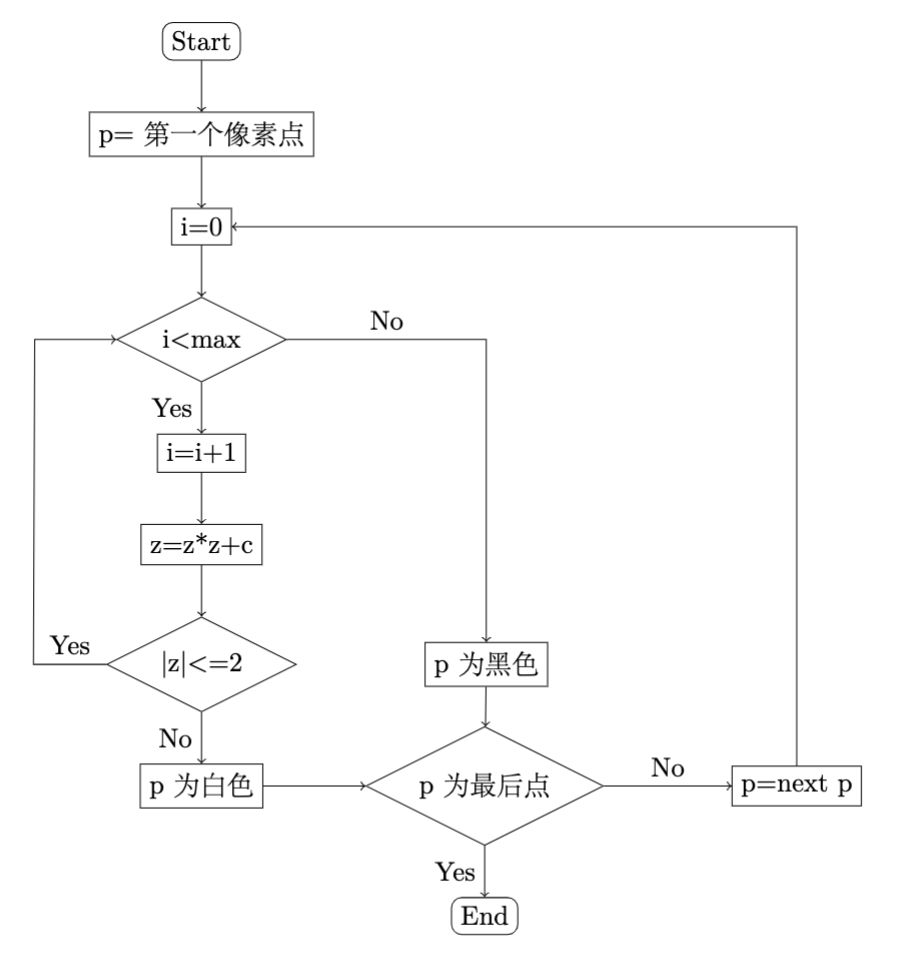
\includegraphics[width=5cm]{../../pic/algorithm.png}
            \end{figure}
        \end{column}
    \end{columns}
\end{frame}

\section{数值算例}
\subsection{性质研究}
\begin{frame}{性质研究}
更改迭代复常数$c$为(0.38,-0.249)并对其进行局部细节的放大可得以下图像:
\begin{columns}
    \column{.5\textwidth}
    \begin{figure}[H] 
    \centering 
    \includegraphics[width=0.85\textwidth]{../../pic/pic2.bmp} 
    \caption{dim=2,c=0.38-0.249i} 
    \end{figure}
    \column{.5\textwidth}
    \begin{figure}[H] 
    \centering 
    \includegraphics[width=0.85\textwidth]{../../pic/pic3.bmp} 
    \caption{dim=0.01,c=0.38-0.249i} 
    \end{figure}
\end{columns}
对于朱利亚集合图像任意倍数放大,仍然保留有着无限精细的结构,并且图案
具有某种程度上的相似性。由此可见,朱利亚集合和曼德博集合相似,具有分形图形的以下两个性质:
\begin{itemize}
    \item 自相似性,即整体与局部以某种方式相似
    \item 边界无限精细
\end{itemize}
\end{frame}

\subsection{关联性研究}
\begin{frame}{关联性研究}
由《分形几何》\cite{1997Techniques}中阐述的理论,使朱利亚集合联通的迭代复常数点应该属于曼德博集合,
选取两个迭代复常数分别属于曼德博集合以及它的补集,分别得到以下两个朱利亚集合的图像,
由图\ref{pic::4},\ref{pic::5}的图像性质得以验证上述结论。
\begin{columns}
    \column{.5\textwidth}
    \begin{figure}[H]
        \centering
        \includegraphics[width=0.33\textwidth]{../../pic/pic4.bmp}
        \caption{c=0.38-0.249i}
        \label{pic::4}
    \end{figure}

    \column{.5\textwidth}
    \begin{figure}[H] 
    \centering 
    \includegraphics[width=0.33\textwidth]{../../pic/pic5.bmp} 
    \caption{c=-0.4+0.6i} 
    \label{pic::5}
    \end{figure}
\end{columns}

将曼德博集合根据形状划分成如图\ref{pic::6}区域,并选取迭代复常数$c$分别在区域1、2中,
则有以下图\ref{pic::7},\ref{pic::8}形状:


\begin{columns}
    \column{.33\textwidth}
    \begin{figure}[H]
        \centering
        \includegraphics[width=3.1cm]{../../pic/pic6.bmp}
        \caption{集合划分}
        \label{pic::6}
    \end{figure}

    \column{.33\textwidth}
    \begin{figure}[H] 
    \centering 
    \includegraphics[width=0.85\textwidth]{../../pic/pic7.bmp} 
    \caption{c=0.1+0.3i} 
    \label{pic::7}
    \end{figure}

    \column{.33\textwidth}
    \begin{figure}[H] 
    \centering 
    \includegraphics[width=0.85\textwidth]{../../pic/pic8.bmp} 
    \caption{c=-1} 
    \label{pic::8}
    \end{figure}
\end{columns}

\begin{itemize}
    \setlength{\itemsep}{1pt}
    \item $c$在1区域内,集合边界为简单闭曲线,有吸引不动点
    \item $c$在2区域内,图像全部由四叉点组成,有吸引2周期轨。
\end{itemize}
事实上,由于曼德博集合所具有的分形性质,这种区域的划分可以无限进行下去。

\end{frame}


\section{结论}
\begin{frame}{结论}
根据以上的算法以及算例分析,不难得到以下结论:
\begin{itemize}
    \setlength{\itemsep}{2pt}
    \item 朱利亚集合性质
    \begin{itemize}
        \item 与曼德博集合类似,由简单递推公式得来,具有分形性质
        \item 对图像放大任意倍数后,仍然具有精细的分形结构和递归细节
    \end{itemize}
    \item 与曼德博集合联系
    \begin{itemize}
        \item 集合图像与$c$相关:当c属于曼德博集合时,朱利亚集合为联通点集
        \item 图像类型与$c$所属的曼德博集合的区域位置有关,具体可根据图像特性无限划分区域
    \end{itemize}
\end{itemize}
\par
事实上,朱利亚集合与曼德博集合就是一个四维分形在不同方向上的二维切片。
\end{frame}

\section{参考文献}

\begin{frame}{参考文献}
    \bibliography{../ref}
    \tiny\bibliographystyle{unsrt}
    % 如果参考文献太多的话,可以像下面这样调整字体:
    % \tiny\bibliographystyle{alpha}
\end{frame}

\end{document}